\chapter{Background}
	\label{CH_02}

This chapter describes the context in which my research makes advances. Section~\ref{gametheory} lays out the basics of game theory. Section~\ref{logic_foundation} introduces Dynamic Epistemic Logic, upon which the logic presented in this thesis is based. Section~\ref{fm} describes the state of formal methods.

%Section 2.3 describes related work involving logical approaches to agents in system verification. Section 2.4 describes the Coq Proof Assistant, a tool for constructing mechanically checked mathematical proofs, to be used in this research.



\section{Game Theory}~\label{gametheory}
Game theory is a mathematical model for strategic reasoning. Strategic reasoning refers to the way an agent reasons in situations where her payoffs depend on the actions of other agents in addition to her own, and in which she knows about these dependencies. For turn-based games, the mathematical structure employed is a \emph{game tree}, where each node represents a player's turn, and each edge the transition via a player's action. The leaves of the tree represent the payoffs each player receives at the end of the game. This paper is not concerned with the games themselves, but rather with the underlying assumptions about agency that entail their solutions. We briefly illustrate these underlying assumptions with the following example.

%Prisoner's Dilemma Matrix
%\begin{table}[!ht]
%	\centering	
%  	\setlength{\extrarowheight}{2pt}
%  	\begin{tabular}{*{4}{c|}}
%  		\multicolumn{2}{c}{} & \multicolumn{2}{c}{Player $B$}\\\cline{3-4}
%  		\multicolumn{1}{c}{} &  & $Cooperate$  & $Defect$ \\\cline{2-4}
%  		\multirow{2}*{Player $A$}  & $Cooperate$ & $(2,2)$ & $(10,0)$ \\\cline{2-4}
%  		& $Defect$ & $(0,10)$ & $(6,6)$ \\\cline{2-4}
%  	\end{tabular}
%\end{table}
\begin{figure}[ht]~\label{tree_ex}
	\begin{center}
		\small
		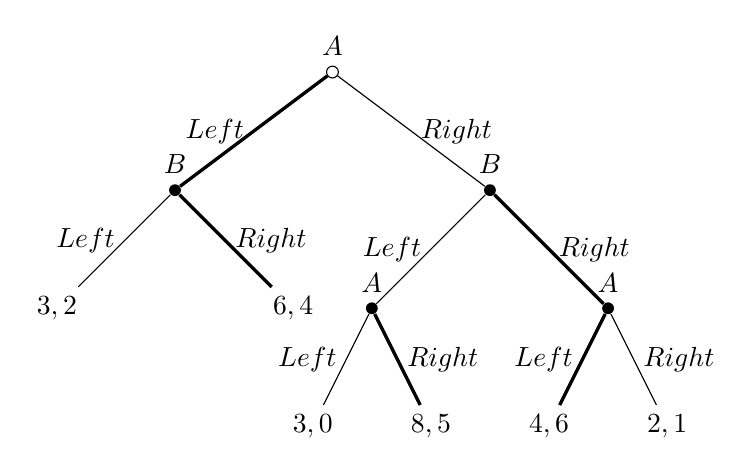
\begin{tikzpicture}[thin,
		level 1/.style={sibling distance=40mm},
		level 2/.style={sibling distance=30mm},
		level 3/.style={sibling distance=15mm},
		every circle node/.style={minimum size=1.5mm,inner sep=0mm}]
		
		\node[circle,draw,label=above:$A$] (root) {}
		child { node [circle,fill,label=above:$B$] (node-F) {}
			child { 
				node {$3,2$}
				edge from parent
				node[left] {$Left$}}
			child { 
				node (node-G) {$6,4$}
				edge from parent
				node[right] {$Right$}}
			edge from parent
			node[left] {$Left$}}
		child { node [circle,fill,label=above:$B$](node-E) {}
			child { 
				node[circle,fill,label=above:$A$](node-B) {}
				child {
					node {$3,0$}
					edge from parent
					node[left] {$Left$}}
				child {
					node (node-A) {$8,5$} 
					edge from parent
					node[right] {$Right$}}
				edge from parent
				node[left] {$Left$}}
			child { 
				node[circle,fill,label=above:$A$](node-C)  {}
				child {
					node (node-D) {$4,6$}
					edge from parent
					node[left] {$Left$}}
				child {
					node {$2,1$}
					edge from parent
					node[right] {$Right$}}
				edge from parent
				node[right] {$Right$}}
			edge from parent
			node[right] {$Right$}};
		\draw [very thick] (node-A) -- (node-B) 
		node[midway,above] {};
		\draw [very thick] (node-C) -- (node-D) 
		node[midway,above] {};
		\draw [very thick] (node-E) -- (node-C) 
		node[midway,above] {};
		\draw [very thick] (node-F) -- (node-G) 
		node[midway,above] {};
		\draw [very thick] (root) -- (node-F) 
		node[midway,above] {};
		\end{tikzpicture}
	\end{center}
	\caption{A game between players A and B}
\end{figure}

We can see in the figure below that the first player to act is Player A, at the root node. Her choices are to move \emph{Left} or \emph{Right}. Player B faces similar choices at the resulting nodes, and the players alternate turns until the game ends and they receive their payoffs, listed \emph{(A,B)}. Briefly glancing through the outcomes, it looks like A should aim for the node with payoff \emph{(8,5)}, because 8 is the highest payoff available to A. However, the official solution to the game is for A to first go \emph{Left}, and then for B to go \emph{Right}, resulting in a payoff of \emph{(6,4)}, where both get less than the intuitively appealing outcome! Why is this so?

Game theory makes strong assumptions about agent knowledge and rationality. The solution to this game is reached through an algorithm called \emph{backward induction}~\cite{VB_TowardPlay}. The players reason by starting at each end node and looking to the immediate parent node, and asking what the deciding player will do at that node, assuming she will choose the path with the highest payoff. So, at the bottom right of the figure, player A is to act, and she can go \emph{Left} for a payoff of 4, or \emph{Right} for a payoff of 2. So, she will go \emph{Left}, illustrated by the bold line. The end nodes not selected are subsequently eliminated. This process is repeated at each end node. Then it is recursively applied up the tree. So along the right branch, player B decides between \emph{Left} for a payoff of 5, or \emph{Right} for a payoff of 6, because B knows that A is rational, and he knows how she will act at each end node. A, at the root, then must choose between \emph{Left} for a payoff of 6, or \emph{Right} for a payoff of 4, because she knows that B is rational, and knows that B knows that she is rational. The explanation begins to illustrate the assumptions game theory makes about each player's knowledge. In fact, this only scratches the surface.

%The story is that Players A and B have been arrested for committing a crime together, and the prosecuting attorney offers them each the following deal: You and your partner in crime can either Defect from or Cooperate with each other. If you Defect and she Cooperates, I will let you go free, and come down hard on her with 10 years. If you both Defect, you will each get 6 years. If you both Cooperate with each other, I can only convict you of a lesser crime, which carries a sentence of 2 years. Some tellings assert that the defendants cannot communicate, but this does not matter under the classical model of rationality. No matter what the other does, each agent is better off by Defecting. Thus, the rational outcome of the game is for each agent to defect, each receiving 6 years. The counterintuitive aspect here is that if each agent have Cooperated, then they collectively would have been better off with 2 years each. But, this outcome cannot occur, because if one Cooperates, the other should Defect: 0 years is better than 2 years.

Game theory, and classical economics in general, makes the following assumptions about agent knowledge, formalized in epistemic logic~\cite{Aumann}. 

$\mathbf{Agency\  Model\  in\  Classical\  Game\  Theory}$.\\
(1) $\Kns{i}(\varphi \iimplies \psi) \iimplies (\Kns{i}\varphi \iimplies \Kns{i}\psi)$\\
(2) $\Kns{i}\varphi \iimplies \varphi$\\
(3) $\Kns{i}\varphi \iimplies \Kns{i}\Kns{i}\varphi$\\
(4) $\tlnot \Kns{i}\varphi \iimplies \Kns{i}\tlnot\Kns{i}\varphi$\\
(5) $\mathbf{C}_G ((1) \tland (2) \tland (3) \tland (4) \tland (5))$.

This forms an idealized model of the knowledge component of classical game theory's agents. $\Kns{i}$ is a modal operator for knowledge, and $\Kns{i}\varphi$ reads, ``agent \emph{i} knows that $\varphi$." $\mathbf{C}_G$ is a modal operator for common knowledge, the fixpoint for ``everyone in group G knows that everyone knows that..." The agents are logically omniscient due to (1), knowledge implies truth with (2), agents have \emph{positive introspection} with (3), and \emph{negative introspection} with (4). Assumptions (1), (3), (4), and (5) are somewhat dubious. The model also fails to formally represent other aspects of agency, like action and evaluation of outcomes. The model we propose makes weaker, more realistic assumptions about knowledge, includes a modal operator for belief, and formally represents action and the evaluation of actions as either safe or unsafe.

Recent work at the intersection of game theory and logic focuses on the information flow that occurs during games. Van Ditmarsch identifies a class of games called \emph{knowledge games}, in which players have diverging information~\cite{ditmarsch}. This slightly relaxes the assumption of classical game theory that players have common knowledge about each other's perfect information. Similarly, it invites logicians to study the information conveyed by the fact that an action is executed. For example, if the action is that agent $1$ asks agent $2$ the question, ``$p$?", the information conveyed is that $1$ does not know whether $p$, believes that $2$ knows whether $p$, and after the action occurs, this information becomes publicly known. The logic modeling games of this kind is of particular interest to us, as we are concerned with identifying the knowledge and belief state of human pilots based on their actions. 

The proceeding sections introduce the various logical systems that form a foundation for the work of this thesis, starting with modal logic in its traditional philosophical interpretation, and expanding to epistemic and doxastic logic. Then, we introduce dynamic logic, and its expansion into Dynamic Epistemic Logic and Public Announcement Logic.

\section{Modal Logic}
Philosophers seek to study not just empirical facts of the actual world, but also necessary truths that hold both in the actual world and in all worlds that might exist. Examples of necessary truths are those of mathematics, which do not depend on any contingent facts of the world in order to be true. The definitions of natural numbers and the the addition function guarantee that in all possible worlds, \emph{2 + 2 = 4}. Modal logic allows us to reason about necessary, possible, and actual truths, through the use of modal operators. What follows is a brief illustration of the concepts and example proofs in modal logic.

Suppose $p$ is the aforementioned arithmetic expression. Obviously, $p$ is true in the actual world. We can make the stronger claim that $p$ is necessarily true, that is, true in all possible worlds, with the modal operator for necessity: $\Box p$. We can explore our first modal inference with these two components: $\Box p \iimplies p$. If $p$ is necessarily true, is it true? Intuitively, the answer is `yes', and indeed a modal logic of metaphysical necessity includes this axiom for all formulas $\varphi$: $\Box \varphi \iimplies \varphi$. 

What other inferences can we make, based on our intuitive notion of necessity and possibility? What about ``if $p$ is true, then $p$ is possibly true"? To formalize this, we need the modal operator for possibility: $\Diamond$. So, the modal formula would be $p \iimplies \Diamond p$. This seems true as well, and indeed it is an axiom: $\varphi \iimplies \Diamond \varphi$. In fact, those two axioms are equivalent. The definition of $\Diamond \varphi \equiv \tlnot \Box \tlnot \varphi$, for any arbitrary formula $\varphi$. This states that something is possible if and only if it is not necessarily false. It can also be said that something is necessary if and only if it is not possibly false: $\Box \varphi \equiv \tlnot \Diamond \tlnot \varphi$. We can now prove that the two axioms are equivalent.

\begin{proof}
	We first prove $\Box \varphi \iimplies \varphi$ implies $\varphi \iimplies \Diamond \varphi$, for any arbitrary $\varphi$ so long as it is the same on each side of the $\iimplies$. We begin by assuming $Box \varphi \iimplies \varphi$. By the definition of $\Box$, we can substitute the equivalent formula $\tlnot \Diamond \tlnot \varphi \iimplies \varphi$. By contraposition, it holds that $\tlnot \varphi \iimplies \Diamond \tlnot \varphi$. But $\varphi$ is any arbitrary formula, including $\tlnot \varphi$. So we can substitute arbitrary formulas and get $\varphi \iimplies \Diamond \varphi$. What matters is that the $\varphi$ on the left and right of the $\iimplies$ are the same, not that they are the same in each axiom.
	
	Next we prove that $\varphi \iimplies \Diamond \varphi$ implies $\Box \varphi \iimplies \varphi$, for arbitrary $\varphi$'s in each axiom. Assume $\varphi \iimplies \Diamond \varphi$. We can substitute in the equivalent formula using the definition of $\Diamond$ and get $\varphi \iimplies \tlnot \Box \tlnot \varphi$. By contraposition, it follows that $\Box \tlnot \varphi \iimplies \tlnot \varphi$. We substitute in $\varphi$ for $\tlnot \varphi$ as the arbitrary formula, and have $\Box \varphi \iimplies \varphi$.
\end{proof}

It is obvious then that $\Box \varphi \iimplies \Diamond \varphi$ is a theorem. This states that if something is necessarily true then it is possibly true. What about the other direction: $\Diamond \varphi \iimplies \Box \varphi$? It turns out this is not a theorem under the typical notions of necessity and possibility. But this raises a question about how we would present a counterexample that disproves it. To do this, we need a semantics for the logic. The semantics we use are called \emph{possible world semantics}, and they are due to Saul Kripke~\cite{Kripke}. One would be hard-pressed to find a species of modal logic, whether in economics, computer science, or philosophy, that does not use possible world semantics in some form or another. Sometimes they are referred to as \emph{Kripke semantics}.

In possible world semantics, a graph structure is created with worlds as nodes and accessibility relations among worlds as the edges in the graph. Propositional formulas are true or false at each world. These graph structures are typically called Kripke structures. We can define the following Kripke structure, $\mathcal{M} = \{W, R, V\}$, where $W$ is a finite set of worlds, $\{w, v\}$, $R$ is a binary accessibility relation defined on those worlds $\{(w,v), (v,w)\}$, meaning $w$ has access to $v$ and $v$ has access to $w$, and $V$ is a \emph{valuation} function, which maps propositions to sets of worlds at which they are true. For example, if $p$ is true at $w$, then $w \in V(p)$. In our model we only care about the proposition $p$, which now stands for some contingent proposition, like ``all swans are white". Formally, we say $w \not\in V(p)$ if not all swans are white in world $w$, denoted by $\tlnot p$, while $w \in V(p)$ if they are, denoted by $p$. The following figure illustrates $\mathcal{M}$:

\begin{figure}[H]
	\begin{center}
	\begin{tikzpicture}[->,>=stealth',shorten >=1pt,auto,node distance=3cm,
	thick,base node/.style={circle,draw,minimum size=35pt}]
	
	\node[base node] (w) {$w: \tlnot p$};
	\node[base node] (v) [right of=w] {$v: p$};
	\path[]
	(w) edge node[above] {$R$} (v)
	    edge [loop left] node {$R$} (w)
	(v) edge node[below] {} (w)
%	\draw [->] (v) edge[in=5,out=355,loop] node[right] {$R$} (v)
	    edge [<-, loop right] node {$R$} (v);
	\end{tikzpicture}
	\end{center}
	\caption{$\mathcal{M}$: A simple counterexample using possible world semantics.}
\end{figure}

According to possible world semantics, $\Box \varphi$ is true at a world, written $w \models \Box \varphi$ for world $w$, if and only if for all worlds $v$ such that $R(w,v)$ ($v$ is accessible to $w$ by the $R$ relation), $v \models \varphi$. This says a formula is necessarily true at a world if and only if it is true at all worlds accessible by that world. Similarly, $w \models \Diamond \varphi$ if and only if there is some world $v$ such that $R(w,v)$ and $v \models \varphi$. In $\mathcal{M}$, $w$ is $R$-accessible to itself, so there is a world accessible to $w$ where $p$ is false, and thus $w \models \tlnot \Box p$. However, since $v$ is $R$-accessible to $w$, and $v \models p$, it is true that $w \models \Diamond p$. Thus, we have $w \models \Diamond p$ and $w \models \tlnot \Box p$, a negation of $\Diamond p \iimplies \Box p$, so it cannot be the case that $\Diamond \varphi \iimplies \Box \varphi$ is a theorem, for arbitrary formula $\varphi$.

While introducing the concepts and what proofs look like in modal logic, syntax and semantics have been alluded to sporadically, but I have not yet formally defined them. I do that here, having properly motivated them.

\section{Modal Logic Syntax and Semantics}~\label{molo_syn_sem}
This section formally defines the syntax, what the logic looks like, and the semantics, what the truth conditions are for the logic. Before looking at the syntax for modal logic, we examine that of Boolean propositional logic.

Recall that Boolean logic is a simple logic for reasoning about basic propositions using the logical connectives `and', `or', `not', and `if...then'. It forms the foundation of most logics and has applications ranging from philosophy to circuit design. Propositions are represented as constants {\emph p,\ \emph q} and well-formed formulas of the language are constants and any proper combination of constants using the above logical connectives, represented symbolically as,
$$\varphi \stackrel{def}{=} p\  |\  \varphi \wedge \varphi\  |\  \varphi \vee \varphi\  |\ \neg \varphi \ |\   \varphi \rightarrow \varphi. 
$$

As illustrated in the previous section, modal logic adds to propositional logic with modal operators for necessary and possible truths. The syntax for propositional logic is extended in the following way:
$$\varphi \stackrel{def}{=} p\  |\  \varphi \wedge \varphi\  |\  \varphi \vee \varphi\  |\ \neg \varphi \ |\   \varphi \rightarrow \varphi\ |\ \Box \varphi \ |\ \Diamond \varphi. 
$$

The semantics for Boolean logic are simply truth tables for each connectives, which I will not reproduce here. Because the connectives are truth-functional, truth tables suffice. However, the operators in modal logic are not truth functional, and require more complex semantics, which we earlier mentioned are called possible world semantics. They are as follows.

For a Kripke model $\mathcal{M} = \{W, R, V\}$ such that $W$ is a set of possible worlds, $R$ is a binary relation on those worlds, and $V$ is a valuation function mapping truth values to propositions at worlds,  

\begin{align*}
w \models p\  &\mathbf{iff}\ w \in V(p) \\
w \models \neg \varphi\  &\mathbf{iff}\  w\not\models \varphi  \\
w \models \varphi \wedge \psi\ &\mathbf{iff}\ w\models \varphi\ \mathnormal{and}\ w\models \psi \\
w \models \Box \varphi\  &\mathbf{iff}\ \forall v,\ R(w,v)\  \mathnormal{implies}\ v \models \varphi. \\
w \models \Diamond \varphi\ &\mathbf{iff}\ \exists v,\ R(w,v)\ \mathnormal{and}\ v\models \varphi.
\end{align*}

The character of a modal logic is determined by the binary relation on worlds underlying the modal operators. The logic we have thus far examined is one at which every world is accessible to itself by the binary relation. This condition is called a \emph{frame} condition, and the models that satisfy this condition belong to said frame. This frame is called the \emph{reflexive} frame, because its defining condition is that the accessibility relation is a reflexive predicate:
\begin{equation}
\forall x,\ R(x,x)
\end{equation}

Relaxing this condition changes the frame, and in doing so changes the logic. If we remove the reflexivity condition, the above axioms are no longer axioms, and the above theorem no longer holds. This means that we can specify the axioms we want by specifying the frame condition on the accessibility relation. Each frame condition corresponds to a modal logic axiom. In addition to reflexivity, the other common frame conditions are as follows, with their corresponding modal logic axiom:
\begin{itemize}
	\item Transitivity
	\begin{eqnarray}
	\forall x,y,z\ R(x,y) \tland R(y,z) \iimplies R(x,z)\\
	\Box \varphi \iimplies \Box \Box \varphi
	\end{eqnarray}
	\item Symmetry
	\begin{eqnarray}
	\forall x,y\ R(x,y) \iimplies R(y,x)\\
	\varphi \iimplies \Box \Diamond \varphi
	\end{eqnarray}
	\item Euclidean
	\begin{eqnarray}
	\forall x,y,z\ R(x,y) \tland R(y,z) \iimplies R(x,z)\\
	\Diamond \varphi \iimplies \Box \Diamond \varphi
	\end{eqnarray}
	\item Seriality
	\begin{eqnarray}
	\forall x \exists y, R(x,y) \\
	\Box \varphi \iimplies \Diamond \varphi
	\end{eqnarray}
\end{itemize}

We saw earlier that reflexive frames are also serial frames, because we proved that we could derive the axiom for serial frames as a theorem from just the axiom for reflexive frames.
%This is formalized in a couple different ways in the literature, sometimes as we did before mapping a proposition-world pair to a Boolean, sometimes defining propositions as sets of worlds, where $V(w)\in p$ if and only if $p$ is true at world $w$. The former convention will be followed here.



%\subsection{Avionics and Formal Methods}
\section{Logical Framework}~\label{logic_foundation}
%This section introduces the logic used as a tool to formally model and reason about pilots in emergency situations. For most readers the logic to be used will be sufficiently complex and unfamiliar that a gradual approach is warranted, beginning with the basics of familiar Boolean logic, and advancing to the final logic specially developed for reasoning about pilot error.
%\subsection{Logical Foundations} 
Recall that Boolean logic is a simple logic for reasoning about basic propositions using the logical connectives `and', `or', `not', and `if...then'. It forms the foundation of most logics and has applications ranging from philosophy to circuit design. Propositions are represented as constants {\emph p,\ \emph q} and well-formed formulas of the language are constants and any proper combination of constants using the above logical connectives, represented symbolically as,
$$\varphi \stackrel{def}{=} p\  |\  \varphi \wedge \varphi\  |\  \varphi \vee \varphi\  |\ \neg \varphi \ |\   \varphi \rightarrow \varphi. 
$$

Boolean logic is limited in what it can express, however. Some situations require higher fidelity, for example when reasoning about knowledge. Consider the proposition, ``If Alice knows $p$, then $p$ is true." Philosophers of knowledge agree with this proposition, considering it a valid claim about knowledge, based on the principle that all known propositions are true. However, this validity cannot be faithfully represented in propositional logic as a general validity. Each sentence in the claim is assigned its own constant, resulting in a formalization like, ``$\mathit{a} \rightarrow \mathit{p}$," with {\emph a} representing ``Alice knows $p$," and $p$ representing ``$p$ is true." But $\mathit{a} \rightarrow \mathit{p}$ is not a validity of Boolean logic. 

To represent reasoning about knowledge, and other similar domains requiring higher fidelity, epistemic operators are added to the basic Boolean logic, resulting in the following logic:

$$\varphi \stackrel{def}{=} p\  |\ \mathbf{K_{i}}\varphi\ |\ \neg \varphi\ |\ \varphi \wedge \varphi, 
$$
where $\mathbf{K_{i}}\varphi$ states that agent ${\boldmath i}$ \emph{knows} that \emph{$\varphi$}, allowing us to formally represent the above validity:
$$\mathbf{K_{Alice}}p \rightarrow p.$$

Semantics for epistemic logic are given by Kripke structures, which serve as models by which epistemic formulas are evaluated. At its core, a Kripke structure is a graph with nodes and edges, accompanied by a function determining which atomic propositions are true at which worlds. The nodes are normally thought of as possible worlds, or as possible states of the system being modeled. The edges are normally thought of as possibility relations among worlds or states. If, at a node representing a world {\emph w}, agent {\emph A} considers it possible that she is in world {\emph v}, the Kripke semantics modeling this situation would have world {\emph w}'s node connected to world {\emph v}'s node by an edge representing {\emph A}'s epistemic possibility relation.

Formally, we say a Kripke structure is a \emph{tuple} $\langle W,\ V,\ Agents,\ \{R_{i}|i\in Agents\}\rangle,$ where \emph{W} is a set of worlds, \emph{V} is a function from propositional constants to sets of worlds satisfying the proposition, \emph{Agents} is a set of agents, and each $R_{i}$ is agent \emph{i}'s epistemic possibility relation.

The semantics are as follows, for worlds $w,\ v\ \in W$:
\begin{align*}
w \models p\  &\mathbf{iff}\ w \in V(p) \\
w \models \neg \varphi\  &\mathbf{iff}\  w\not\models \varphi  \\
w \models \varphi \wedge \psi\ &\mathbf{iff}\ w\models \varphi\ \mathnormal{and}\ w\models \psi \\
w \models \mathbf{K_{i}}\varphi\  &\mathbf{iff}\ \forall v,\ wR_{i}v\  \mathnormal{implies}\ v \models \varphi.
\end{align*}

Early applications of epistemic logic in information security modeled system components as agents whose knowledge represented the information flowing to them. Recently, a modified version of epistemic logic known as dynamic epistemic logic has been used in information security to formally reason about security properties involving human components of systems. The research described in this proposal advances along similar lines, treating pilots as human components of safety critical aviation systems and using dynamic epistemic logic to reason about them. The next section describes the basic dynamic epistemic logic.

\subsection{Dynamic Epistemic Logic}~\label{delsubsection}
Dynamic Epistemic Logic (DEL) formalizes situations in which agents' epistemic states change over time, due to announcements or other informational events.~\cite{DEL} For example, if Alice truthfully and trustworthily communicates to Bob that $\varphi$, then after this informational even it is true that Bob knows $\varphi$. This situation cannot be modeled by the epistemic logic introduced in the previous section. To model it, we introduce the following formal machinery.

To capture informational events, we introduce the idea of relativizing a Kripke structure. In the previous example, if we model the Alice and Bob situation prior to Alice's communication, we can have a world $w$ from which Bob considers $\varphi$- as well as $\neg\varphi$-worlds possible. However, after the informational event, Bob knows $\varphi$, so the model is \emph{relativized} to a submodel in which only $\varphi$-worlds are accessible by Bob's epistemic possibility relation. Thus, after the informational event, the model transitions to a submodel with fewer edge relations.

The logic for reasoning about information flow in knowledge games is called Dynamic Epistemic Logic (DEL). As its name suggests, it combines elements of epistemic logic and dynamic logic. Epistemic logic is the static logic for reasoning about knowledge, and dynamic logic is used to reason about actions. In dynamic logic semantics, nodes are states of the system or the world, and relations on nodes are transitions via programs or actions from node to node. If we think of each node in dynamic logic as being a model of epistemic logic, then actions become relations on models, representing transitions from one multi-agent epistemic model to another. For example, if we have a static epistemic model $M1$ representing the knowledge states of agents $1$ and $2$ at a moment, then the action $``p?"$ is a relation between $M1$ and $M2$, a new static epistemic model of $1$'s and $2$'s knowledge after the question is asked. All of this is captured by DEL.

\begin {center}
\begin {tikzpicture}[-latex ,auto ,node distance =3 cm and 4cm ,on grid ,
semithick ,
state/.style ={ circle ,top color =white , bottom color = white ,
	draw, text=black , minimum width =1 cm}]

\node[state] (A)  {$M1$};
\node[state] (B) [right =of A] {$M2$};

\path (A) edge  node[above] {$``p?"$} (B);
%\path (C) edge [bend left =25] node[below =0.15 cm] {$1/2$} (A);
%\path (A) edge [bend right = -15] node[below =0.15 cm] {$1/2$} (C);
%\path (A) edge [bend left =25] node[above] {$1/4$} (B);
%\path (B) edge [bend left =15] node[below =0.15 cm] {$1/2$} (A);
%\path (C) edge [bend left =15] node[below =0.15 cm] {$1/2$} (B);
%\path (B) edge [bend right = -25] node[below =0.15 cm] {$1/2$} (C);
\end{tikzpicture}
\end{center}

The above figure illustrates the relationship between static epistemic models and dynamic logic models. As a purely dynamic model, the figure shows the action $``p?"$ transitioning between nodes $M1$ and $M2$. If we were to zoom in on the nodes, we would see their structure as epistemic models, with their own nodes and edges, representing possible worlds and epistemic relations.

We are concerned with an additional element: the \emph{safety} status of an action, and an agent's knowledge and belief about that. To capture this, we extend DEL and call the new logic Dynamic Agent Safety Logic (DASL), which we introduce in the next chapter. The next section lays out the state of formal methods involving human-machine systems.

\section{Formal Methods}~\label{fm}
%The field of formal methods grew out of attempts to verify the correctness of hardware and software. It was normally confined to systems deemed mission- or safety-critical, due to its high cost. Arguments for the use of formal methods normally involve an anecdote in which a system fails due to some sort of error missed by traditional testing methods but that would have been caught and prevented were formal methods used.
Formal methods increase confidence that hardware and software components function correctly~\cite{RushbyFMbook}. They involve the application of mathematical techniques to the design and analysis of systems, usually the safety-critical components~\cite{johnson_butler_fm}. A standard approach is to develop an abstract specification of the software or hardware system, design the system to meet those specifications, and then use formal logic to prove that the designed system meets the desired safety specifications. 

According to the Federal Aviation Administration (FAA), one of the top 12 causes of mistakes in the aviation workplace is a lack of awareness~\cite{faa}. According to Boeing and the FAA, approximately 80 per cent of aviation accidents (including maintenance accidents) are due to human error~\cite{boeing,faaHF}. To increase safety in human factors, the industry relies on education, psychology, anthropometrics, safety engineering, and to a limited extent, computer science. The primary focus of computer science research regarding human factors is the design and testing of software systems that are easy and intuitive for humans to interact with. 

%Formal methods are traditionally deployed in one of two ways. The more painful but perhaps more commonly used approach is to perform \emph{semantic archeology}, wherein an artifact that has already been constructed is formalized into a mathematically rigorous language and then reasoned about. The way urged by most contemporary researchers involves continuously specifying and verifying correctness throughout the development process, prior to system deployment. To facilitate this preferred approach, most formal methods researchers devote themselves to developing tools that are easy to use.
%
%The intended use of these tools, however, has remained the same: to verify the correctness of hardware and software systems, or to provide assistance to mathematicians attempting to prove theorems. At bottom, the tools allow computers to provide assistance to humans who are attempting to prove or disprove mathematical theorems.
%
%Thus we have a situation in which formal methods researchers advocate for the use of formal methods due to the inherent uncertainties involved with empirical testing of systems. However, they are satisfied to leave validation of the human component, the most risky component, to empirical testing.

Some researchers have sought to develop formal methods for mitigating human-induced sources of failure~\cite{ButlerModeConfusion,Rushby_Mode_Confusion}. Thus far this work has focused on the development of formal methods tools for analyzing human machine interaction during the design and specification phase, rather than at runtime. The goals have been to develop software, and techniques for verifying the correctness of that software, to avoid mode confusion, a type of pilot error wherein the pilot believes the autopilot is in one mode, when in reality it is in another. In these situations, the autopilot is not offering protections concerning flight control inputs like thrust and pitch, so the pilot risks providing dangerous inputs.

Butler, Miller, Potts, and Carreno~\cite{ButlerModeConfusion} trace mode confusion to three sources:
\begin{enumerate}
	\item poor display of automation state
	\item unnecessarily complex automation
	\item flight crew has an incorrect mental model of the state of the aircraft
\end{enumerate}

\noindent They say human factors research focuses on mitigating item (1) above, and they develop formal models in the PVS automated theorem prover to address items (2) and (3). However, the formal models they develop are of the automation system, not of the human components.

Similarly, Rushby~\cite{Rushby_Mode_Confusion} describes a class of errors he calls automation surprises, which are distinct but related to mode confusion. These occur when a pilot becomes surprised by the automated behavior of the system. He proposes a formal method addressing automation surprises that constructs a model of the system behavior, constructs a formal specification of a possible pilot's mental model of the system, and compares them for disagreement. His solution focuses on identifying potential automation surprises in the system, and both models are of the system behavior itself: one directly of the model, and one indirectly of the model, mediated through a hypothetical pilot's mind.

In each of the above cases, the formal efforts focus on modeling the system itself, rather than on the human component, and they address the problem at design time. This work complements theirs by constructing a formal model of the pilot herself, and addressing the problem at runtime. Similarly, this work aims to address a variety of problems due to a pilot's loss of situational awareness, including mode confusion. The next chapter introduces Dynamic Agent Safety Logic.